\documentclass{article}
\usepackage[x11names, svgnames, rgb]{xcolor}
\usepackage[utf8]{inputenc}
\usepackage{tikz}
\usetikzlibrary{snakes,arrows,shapes}
\usepackage{amsmath}

\begin{document}
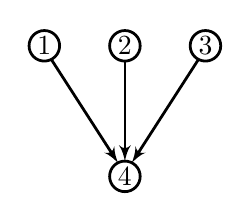
\begin{tikzpicture}[>=latex',line join=bevel,]
  \pgfsetlinewidth{1bp}
%%
\pgfsetcolor{black}
  % Edge: 3 -> 4
  \draw [->] (67.027bp,47.663bp) .. controls (62.447bp,40.556bp) and (52.535bp,25.176bp)  .. (42.966bp,10.327bp);
  % Edge: 1 -> 4
  \draw [->] (13.973bp,47.663bp) .. controls (18.553bp,40.556bp) and (28.465bp,25.176bp)  .. (38.034bp,10.327bp);
  % Edge: 2 -> 4
  \draw [->] (40.5bp,47.021bp) .. controls (40.5bp,40.08bp) and (40.5bp,26.536bp)  .. (40.5bp,10.961bp);
  % Node: 1
\begin{scope}
  \definecolor{strokecol}{rgb}{0.0,0.0,0.0};
  \pgfsetstrokecolor{strokecol}
  \draw (11.5bp,52.5bp) ellipse (5.5bp and 5.5bp);
  \draw (11.5bp,52.5bp) node {1};
\end{scope}
  % Node: 3
\begin{scope}
  \definecolor{strokecol}{rgb}{0.0,0.0,0.0};
  \pgfsetstrokecolor{strokecol}
  \draw (69.5bp,52.5bp) ellipse (5.5bp and 5.5bp);
  \draw (69.5bp,52.5bp) node {3};
\end{scope}
  % Node: 2
\begin{scope}
  \definecolor{strokecol}{rgb}{0.0,0.0,0.0};
  \pgfsetstrokecolor{strokecol}
  \draw (40.5bp,52.5bp) ellipse (5.5bp and 5.5bp);
  \draw (40.5bp,52.5bp) node {2};
\end{scope}
  % Node: 4
\begin{scope}
  \definecolor{strokecol}{rgb}{0.0,0.0,0.0};
  \pgfsetstrokecolor{strokecol}
  \draw (40.5bp,5.5bp) ellipse (5.5bp and 5.5bp);
  \draw (40.5bp,5.5bp) node {4};
\end{scope}
%
\end{tikzpicture}
% End of code

%
\end{document}
%



